\documentclass[11pt]{article}
\usepackage[textwidth=18.0cm, textheight=23.0cm, top=2.0cm]{geometry}
\usepackage{pst-all}
\usepackage{amssymb}
\usepackage{tikz}
\usepackage{underscore}\begin{document}
\pagestyle{empty}


ClassName: \underline{\textbf{Class_05.2bp-11}}
\par
BinSize: \underline{\textbf{100 × 100}}
\par
ReduceSize: \underline{\textbf{100 × 100}}
\par
TypeNum: \underline{\textbf{40}}
\par
Num: \underline{\textbf{40}}
\par
OutS: \underline{\textbf{100000}}
\par
InS: \underline{\textbf{89131}}
\par
Rate: \underline{\textbf{0.891}}
\par
UB: \underline{\textbf{10}}
\par
LB0: \underline{\textbf{10}}
\par
LB: \underline{\textbf{10}}
\par
LBWithCut: \underline{\textbf{10}}
\par
NodeCut: \underline{\textbf{0}}
\par
ExtendedNodeCnt: \underline{\textbf{1}}
\par
GenNodeCnt: \underline{\textbf{1}}
\par
PrimalNode: \underline{\textbf{0}}
\par
ColumnCount: \underline{\textbf{10}}
\par
TotalCutCount: \underline{\textbf{0}}
\par
RootCutCount: \underline{\textbf{0}}
\par
LPSolverCnt: \underline{\textbf{1}}
\par
PricingSolverCnt: \underline{\textbf{0}}
\par
BranchAndBoundNum: \underline{\textbf{1}}
\par
isOpt: \underline{\textbf{true}}
\par
TimeOnInitSolution: \underline{\textbf{0.050 s}}
\par
TimeOnPrimal: \underline{\textbf{0.000 s}}
\par
TimeOnPricing: \underline{\textbf{0.000 s}}
\par
TimeOnRmp: \underline{\textbf{0.047 s}}
\par
TotalTime: \underline{\textbf{0.175 s}}
\par
\newpage


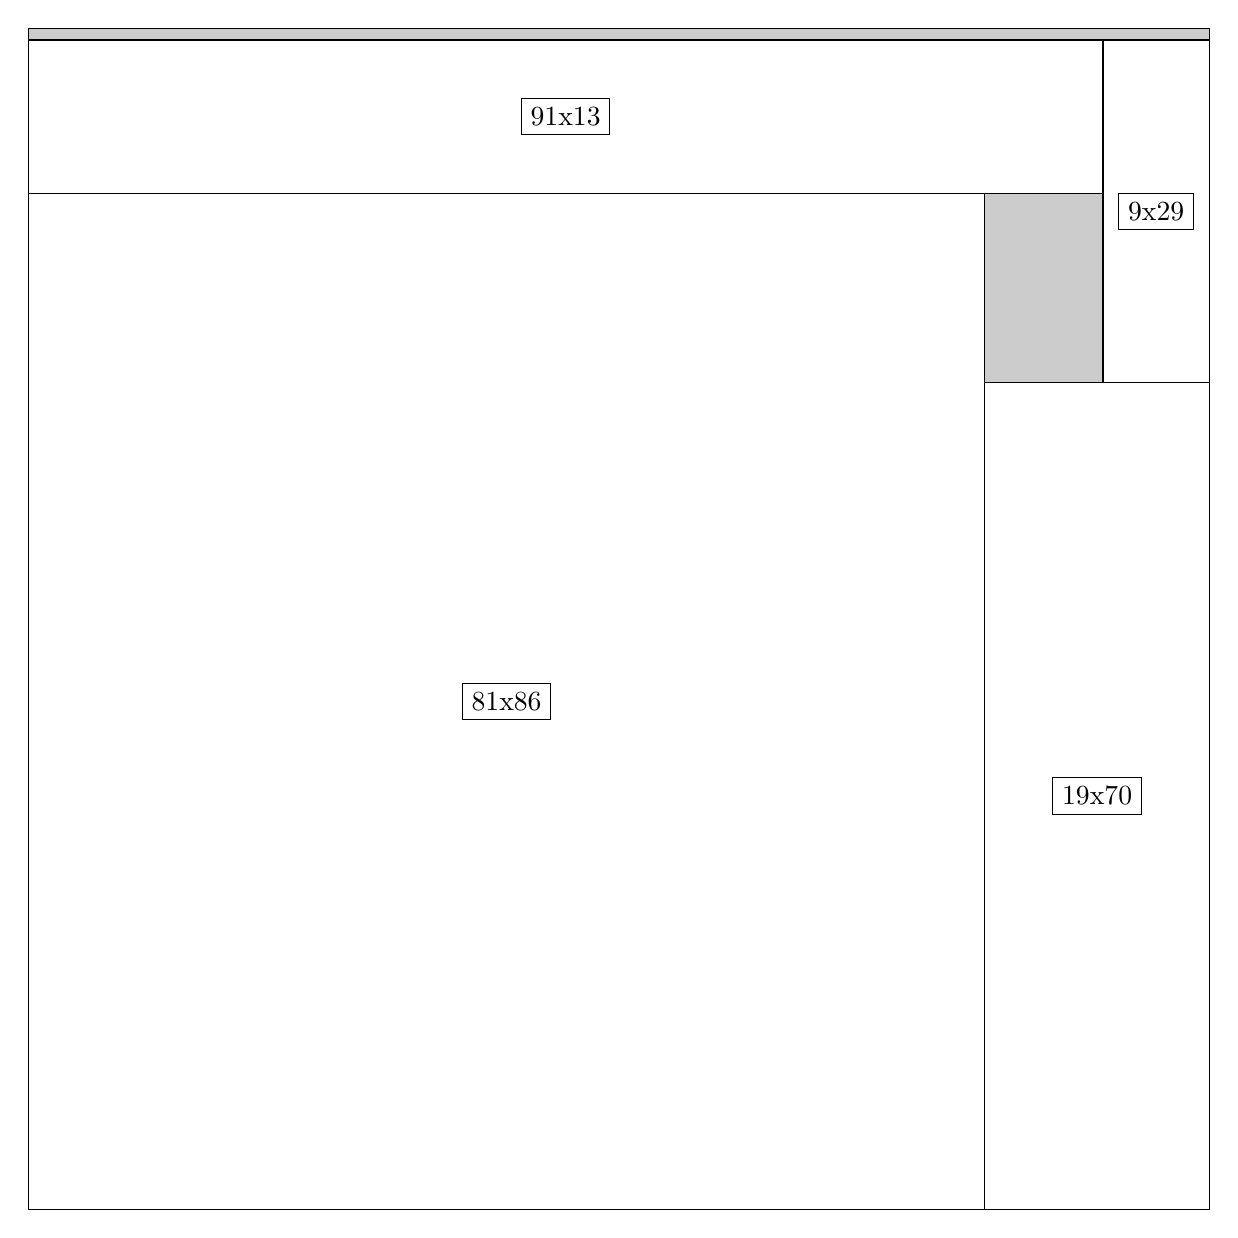
\begin{tikzpicture}[shorten >=1pt,scale=1.0,every node/.style={scale=1.0},->]
\tikzstyle{vertex}=[circle,fill=black!25,minimum size=14pt,inner sep=0pt]
\filldraw[fill=gray!40!white, draw=black] (0,0) rectangle (15.0,15.0);
\foreach \name/\x/\y/\w/\h in {81x86/0.0/0.0/12.15/12.9,19x70/12.15/0.0/2.85/10.5,91x13/0.0/12.9/13.65/1.95,9x29/13.65/10.5/1.3499999999999999/4.35}
\filldraw[fill=white!40!white, draw=black] (\x,\y) rectangle node[draw] (\name) {\name} ++(\w,\h);
\end{tikzpicture}


w =81 , h =86 , x =0 , y =0 , v =6966
\par
w =19 , h =70 , x =81 , y =0 , v =1330
\par
w =91 , h =13 , x =0 , y =86 , v =1183
\par
w =9 , h =29 , x =91 , y =70 , v =261
\par
\newpage


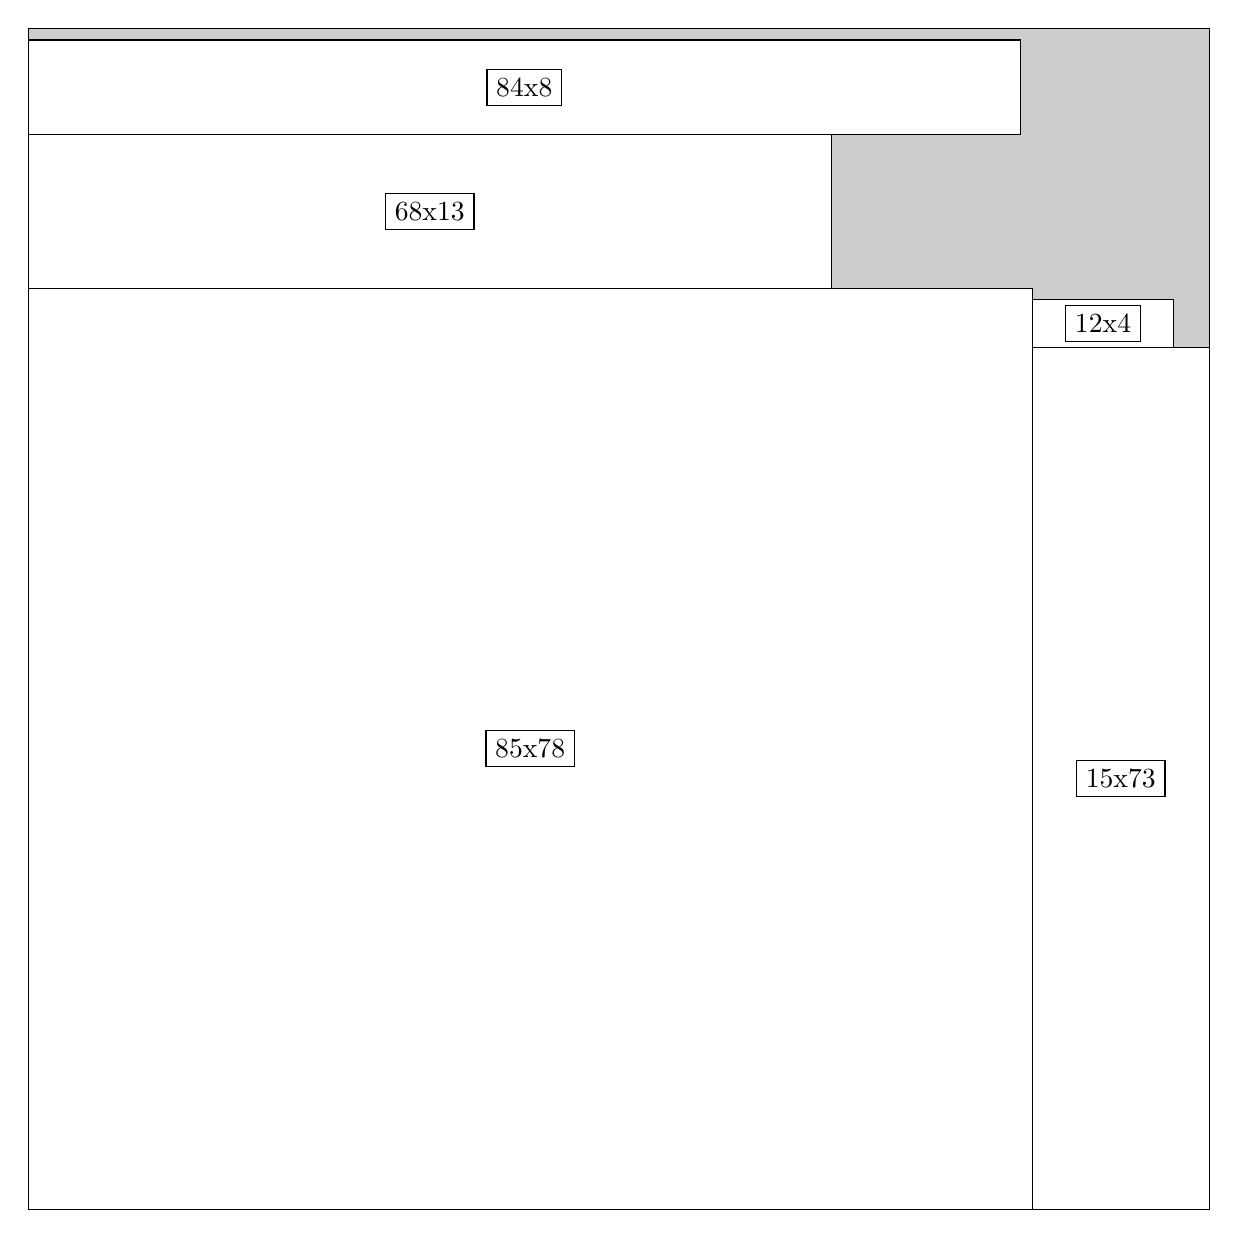
\begin{tikzpicture}[shorten >=1pt,scale=1.0,every node/.style={scale=1.0},->]
\tikzstyle{vertex}=[circle,fill=black!25,minimum size=14pt,inner sep=0pt]
\filldraw[fill=gray!40!white, draw=black] (0,0) rectangle (15.0,15.0);
\foreach \name/\x/\y/\w/\h in {85x78/0.0/0.0/12.75/11.7,15x73/12.75/0.0/2.25/10.95,68x13/0.0/11.7/10.2/1.95,84x8/0.0/13.65/12.6/1.2,12x4/12.75/10.95/1.7999999999999998/0.6}
\filldraw[fill=white!40!white, draw=black] (\x,\y) rectangle node[draw] (\name) {\name} ++(\w,\h);
\end{tikzpicture}


w =85 , h =78 , x =0 , y =0 , v =6630
\par
w =15 , h =73 , x =85 , y =0 , v =1095
\par
w =68 , h =13 , x =0 , y =78 , v =884
\par
w =84 , h =8 , x =0 , y =91 , v =672
\par
w =12 , h =4 , x =85 , y =73 , v =48
\par
\newpage


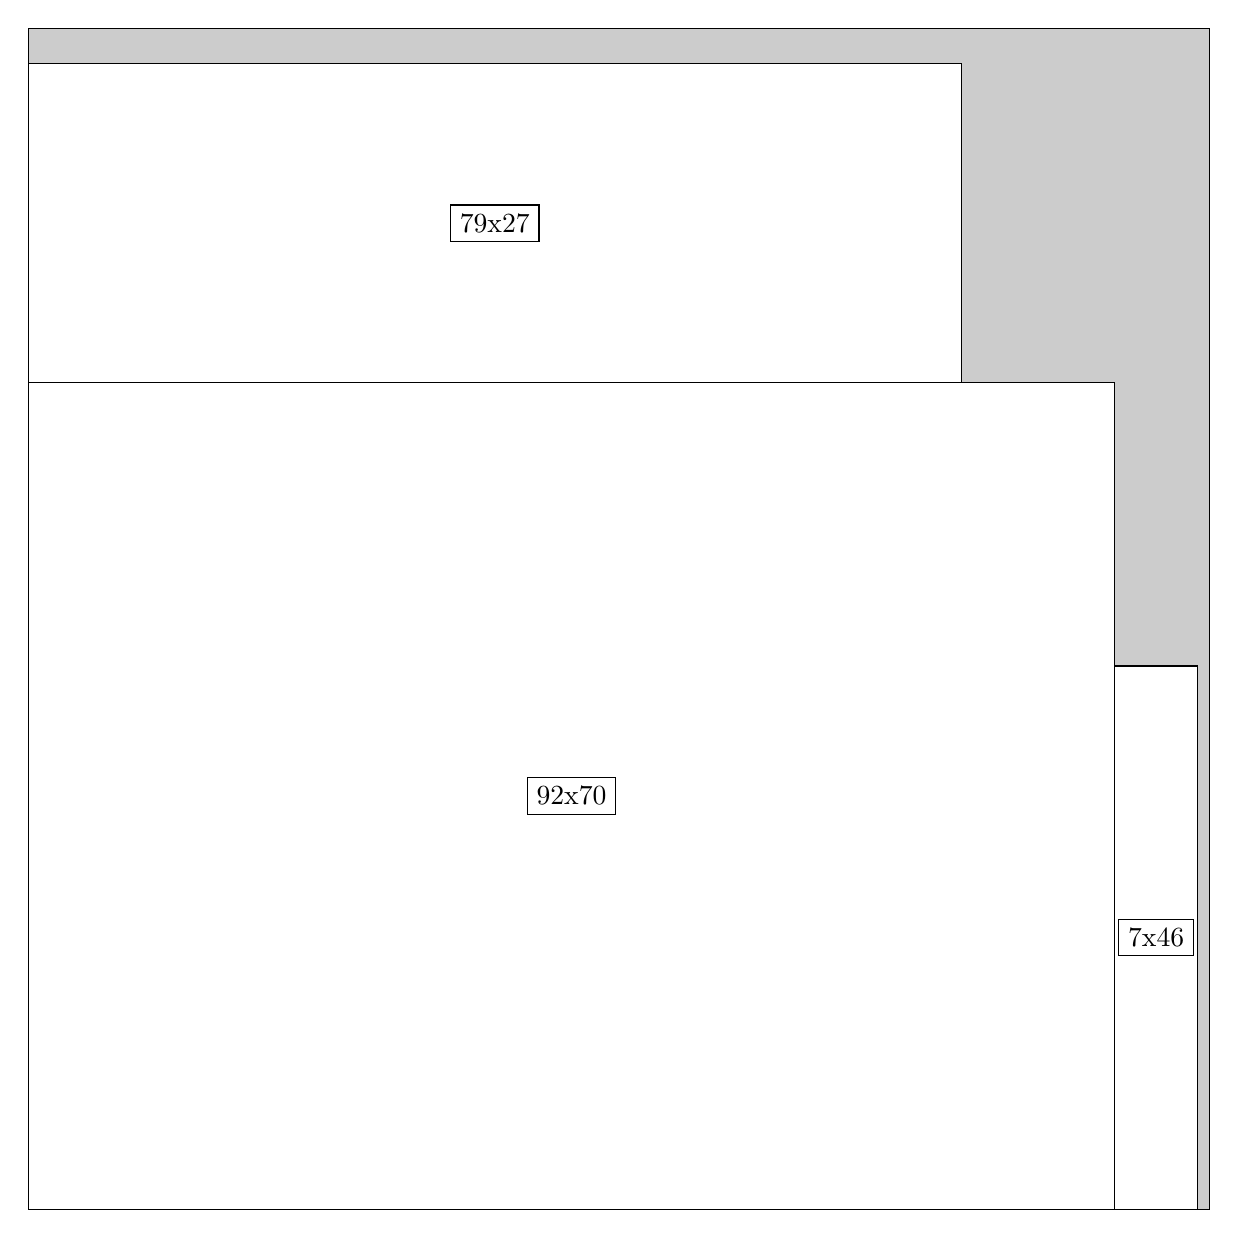
\begin{tikzpicture}[shorten >=1pt,scale=1.0,every node/.style={scale=1.0},->]
\tikzstyle{vertex}=[circle,fill=black!25,minimum size=14pt,inner sep=0pt]
\filldraw[fill=gray!40!white, draw=black] (0,0) rectangle (15.0,15.0);
\foreach \name/\x/\y/\w/\h in {92x70/0.0/0.0/13.799999999999999/10.5,79x27/0.0/10.5/11.85/4.05,7x46/13.799999999999999/0.0/1.05/6.8999999999999995}
\filldraw[fill=white!40!white, draw=black] (\x,\y) rectangle node[draw] (\name) {\name} ++(\w,\h);
\end{tikzpicture}


w =92 , h =70 , x =0 , y =0 , v =6440
\par
w =79 , h =27 , x =0 , y =70 , v =2133
\par
w =7 , h =46 , x =92 , y =0 , v =322
\par
\newpage


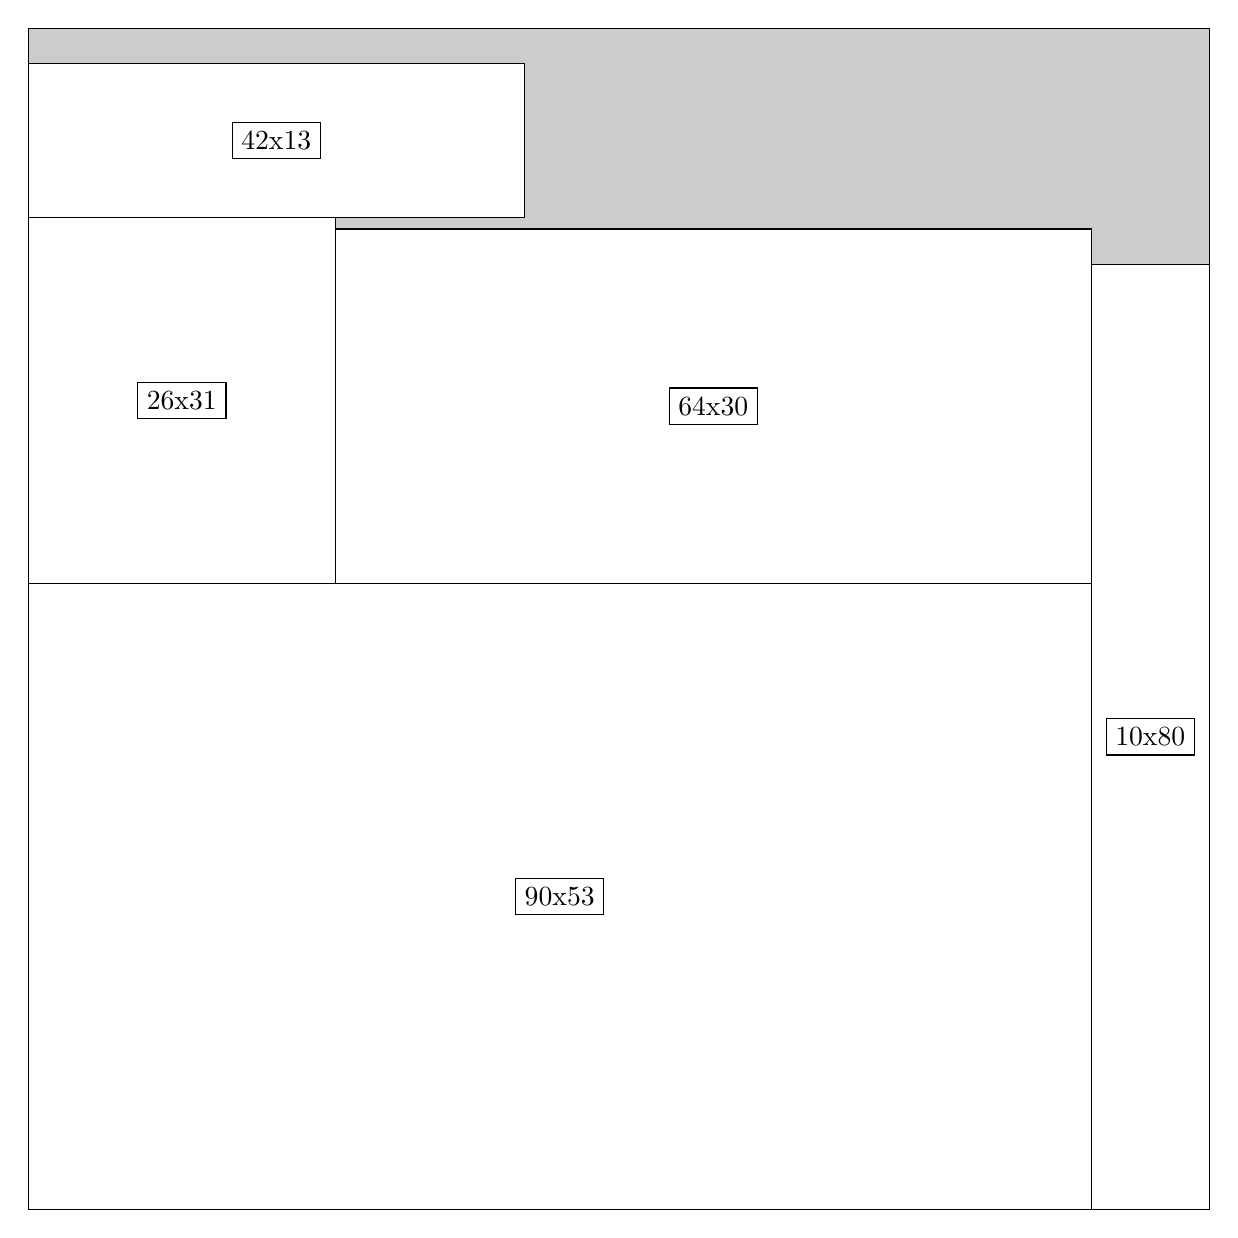
\begin{tikzpicture}[shorten >=1pt,scale=1.0,every node/.style={scale=1.0},->]
\tikzstyle{vertex}=[circle,fill=black!25,minimum size=14pt,inner sep=0pt]
\filldraw[fill=gray!40!white, draw=black] (0,0) rectangle (15.0,15.0);
\foreach \name/\x/\y/\w/\h in {26x31/0.0/7.949999999999999/3.9/4.6499999999999995,64x30/3.9/7.949999999999999/9.6/4.5,90x53/0.0/0.0/13.5/7.949999999999999,10x80/13.5/0.0/1.5/12.0,42x13/0.0/12.6/6.3/1.95}
\filldraw[fill=white!40!white, draw=black] (\x,\y) rectangle node[draw] (\name) {\name} ++(\w,\h);
\end{tikzpicture}


w =26 , h =31 , x =0 , y =53 , v =806
\par
w =64 , h =30 , x =26 , y =53 , v =1920
\par
w =90 , h =53 , x =0 , y =0 , v =4770
\par
w =10 , h =80 , x =90 , y =0 , v =800
\par
w =42 , h =13 , x =0 , y =84 , v =546
\par
\newpage


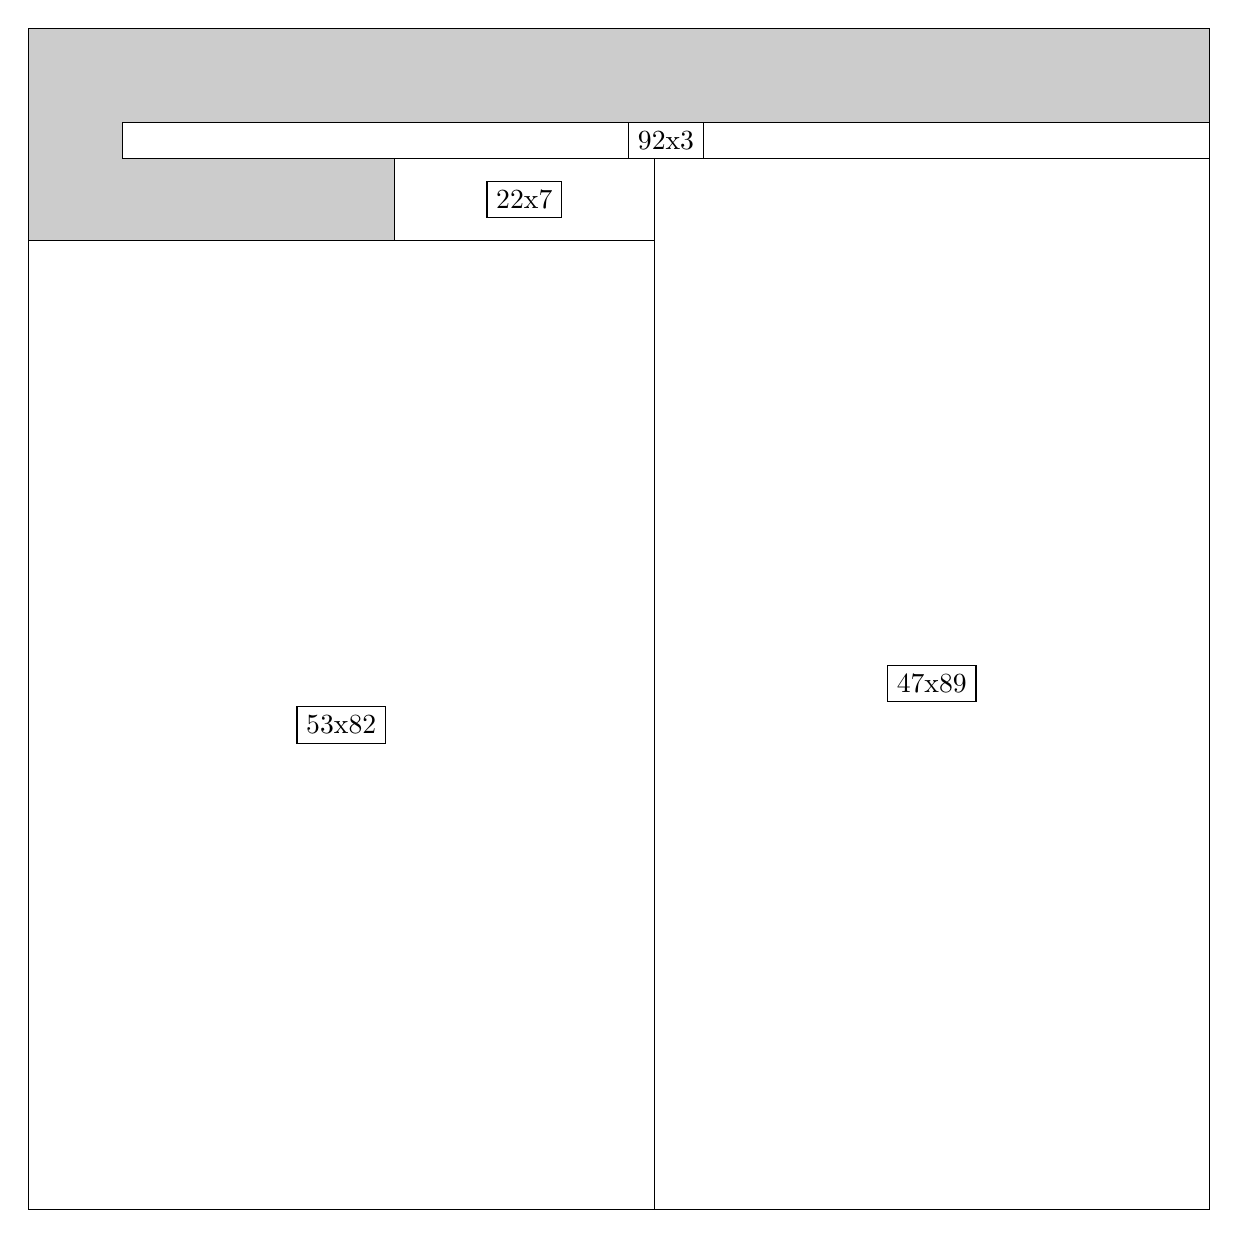
\begin{tikzpicture}[shorten >=1pt,scale=1.0,every node/.style={scale=1.0},->]
\tikzstyle{vertex}=[circle,fill=black!25,minimum size=14pt,inner sep=0pt]
\filldraw[fill=gray!40!white, draw=black] (0,0) rectangle (15.0,15.0);
\foreach \name/\x/\y/\w/\h in {53x82/0.0/0.0/7.949999999999999/12.299999999999999,47x89/7.949999999999999/0.0/7.05/13.35,92x3/1.2/13.35/13.799999999999999/0.44999999999999996,22x7/4.6499999999999995/12.299999999999999/3.3/1.05}
\filldraw[fill=white!40!white, draw=black] (\x,\y) rectangle node[draw] (\name) {\name} ++(\w,\h);
\end{tikzpicture}


w =53 , h =82 , x =0 , y =0 , v =4346
\par
w =47 , h =89 , x =53 , y =0 , v =4183
\par
w =92 , h =3 , x =8 , y =89 , v =276
\par
w =22 , h =7 , x =31 , y =82 , v =154
\par
\newpage


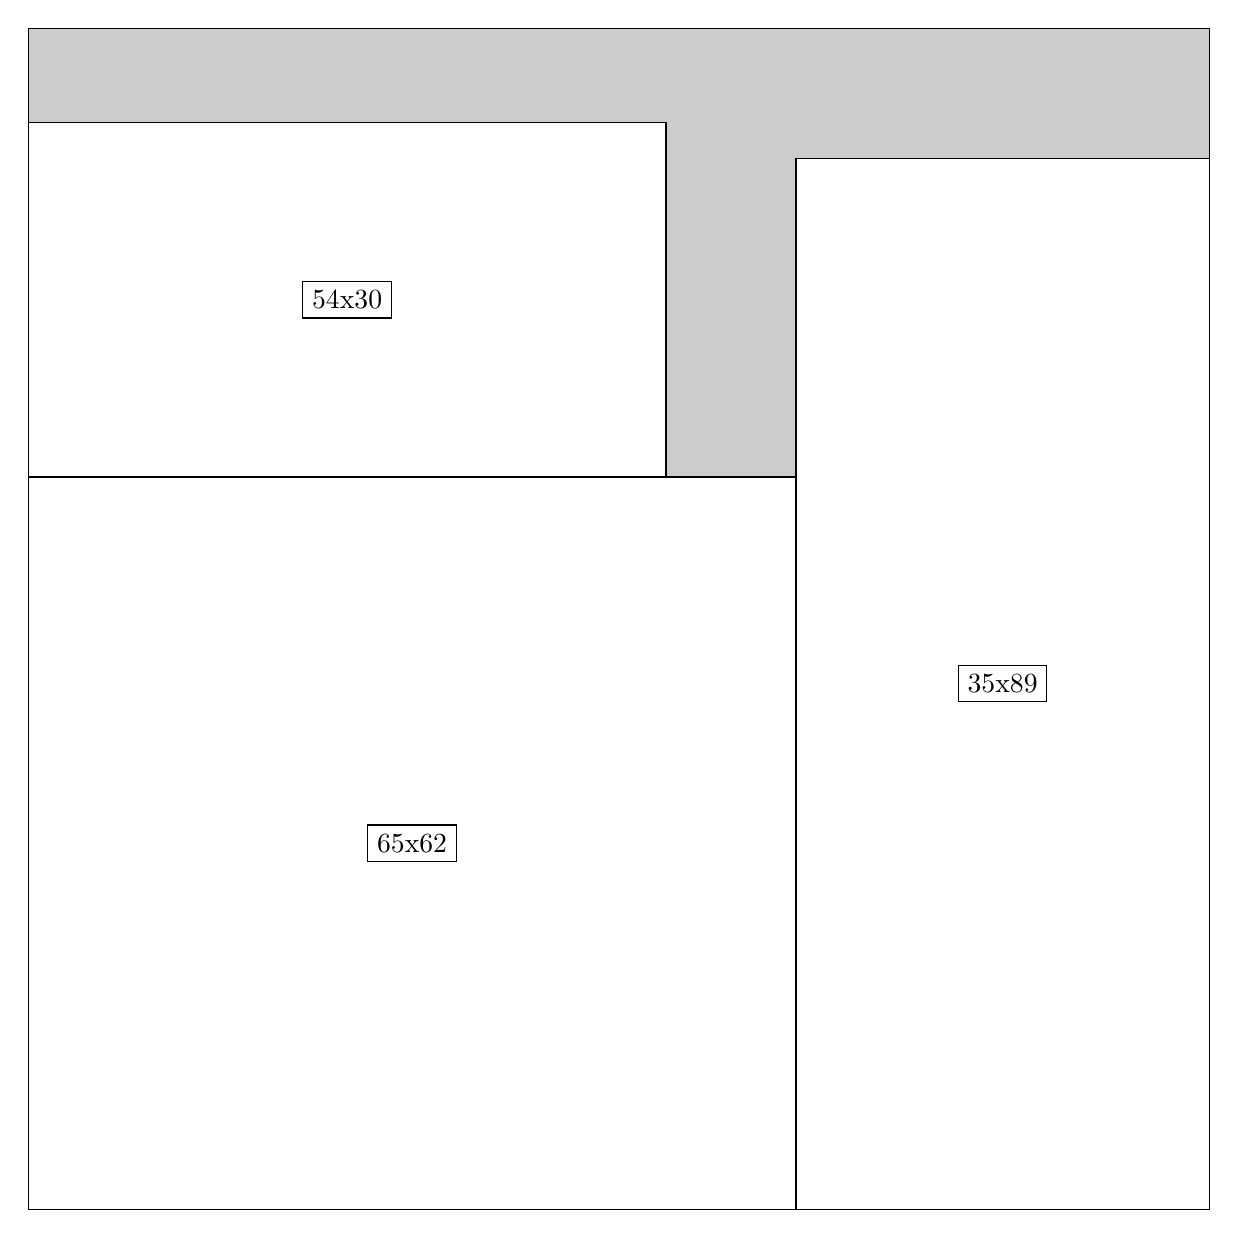
\begin{tikzpicture}[shorten >=1pt,scale=1.0,every node/.style={scale=1.0},->]
\tikzstyle{vertex}=[circle,fill=black!25,minimum size=14pt,inner sep=0pt]
\filldraw[fill=gray!40!white, draw=black] (0,0) rectangle (15.0,15.0);
\foreach \name/\x/\y/\w/\h in {65x62/0.0/0.0/9.75/9.299999999999999,35x89/9.75/0.0/5.25/13.35,54x30/0.0/9.299999999999999/8.1/4.5}
\filldraw[fill=white!40!white, draw=black] (\x,\y) rectangle node[draw] (\name) {\name} ++(\w,\h);
\end{tikzpicture}


w =65 , h =62 , x =0 , y =0 , v =4030
\par
w =35 , h =89 , x =65 , y =0 , v =3115
\par
w =54 , h =30 , x =0 , y =62 , v =1620
\par
\newpage


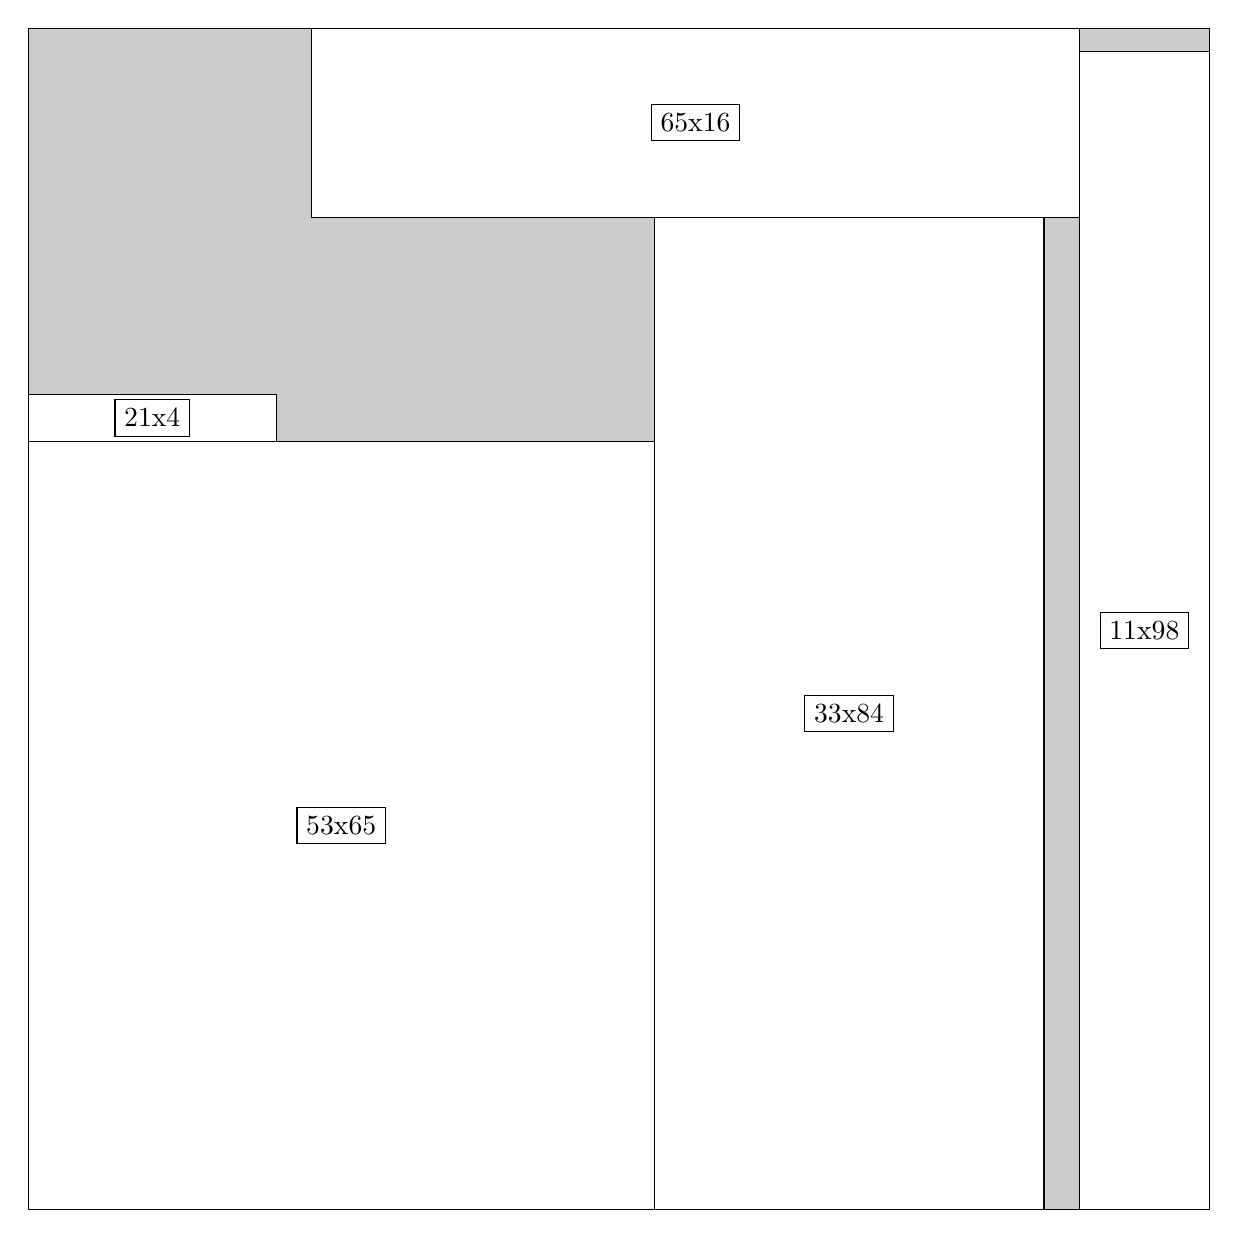
\begin{tikzpicture}[shorten >=1pt,scale=1.0,every node/.style={scale=1.0},->]
\tikzstyle{vertex}=[circle,fill=black!25,minimum size=14pt,inner sep=0pt]
\filldraw[fill=gray!40!white, draw=black] (0,0) rectangle (15.0,15.0);
\foreach \name/\x/\y/\w/\h in {53x65/0.0/0.0/7.949999999999999/9.75,33x84/7.949999999999999/0.0/4.95/12.6,11x98/13.35/0.0/1.65/14.7,65x16/3.5999999999999996/12.6/9.75/2.4,21x4/0.0/9.75/3.15/0.6}
\filldraw[fill=white!40!white, draw=black] (\x,\y) rectangle node[draw] (\name) {\name} ++(\w,\h);
\end{tikzpicture}


w =53 , h =65 , x =0 , y =0 , v =3445
\par
w =33 , h =84 , x =53 , y =0 , v =2772
\par
w =11 , h =98 , x =89 , y =0 , v =1078
\par
w =65 , h =16 , x =24 , y =84 , v =1040
\par
w =21 , h =4 , x =0 , y =65 , v =84
\par
\newpage


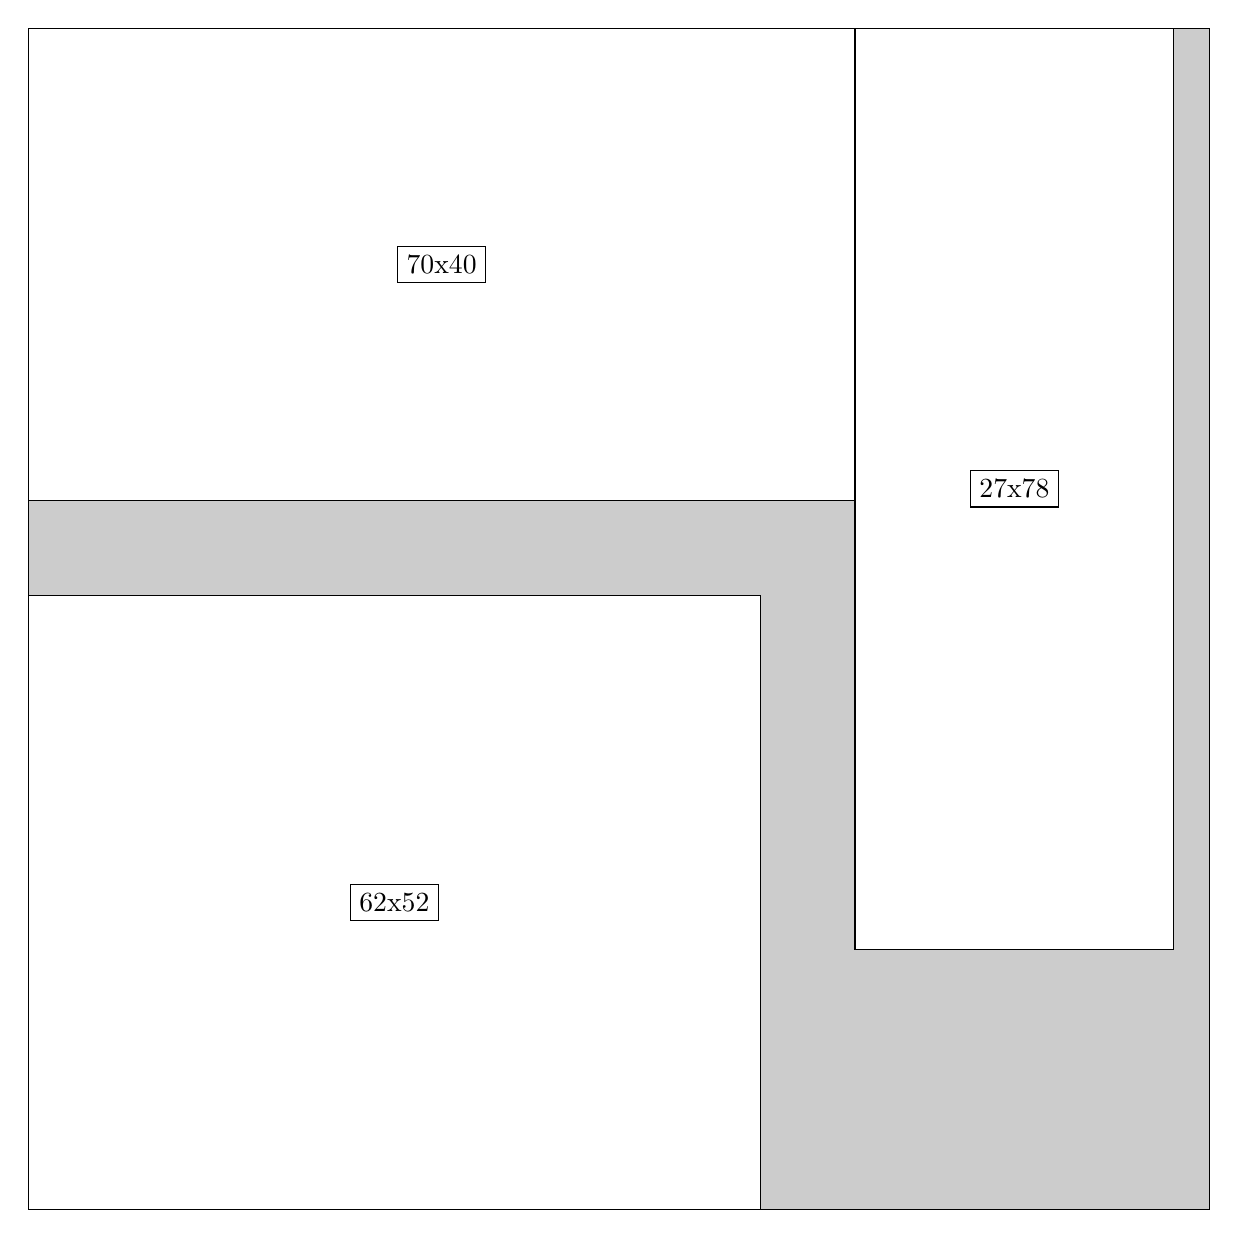
\begin{tikzpicture}[shorten >=1pt,scale=1.0,every node/.style={scale=1.0},->]
\tikzstyle{vertex}=[circle,fill=black!25,minimum size=14pt,inner sep=0pt]
\filldraw[fill=gray!40!white, draw=black] (0,0) rectangle (15.0,15.0);
\foreach \name/\x/\y/\w/\h in {62x52/0.0/0.0/9.299999999999999/7.8,70x40/0.0/9.0/10.5/6.0,27x78/10.5/3.3/4.05/11.7}
\filldraw[fill=white!40!white, draw=black] (\x,\y) rectangle node[draw] (\name) {\name} ++(\w,\h);
\end{tikzpicture}


w =62 , h =52 , x =0 , y =0 , v =3224
\par
w =70 , h =40 , x =0 , y =60 , v =2800
\par
w =27 , h =78 , x =70 , y =22 , v =2106
\par
\newpage


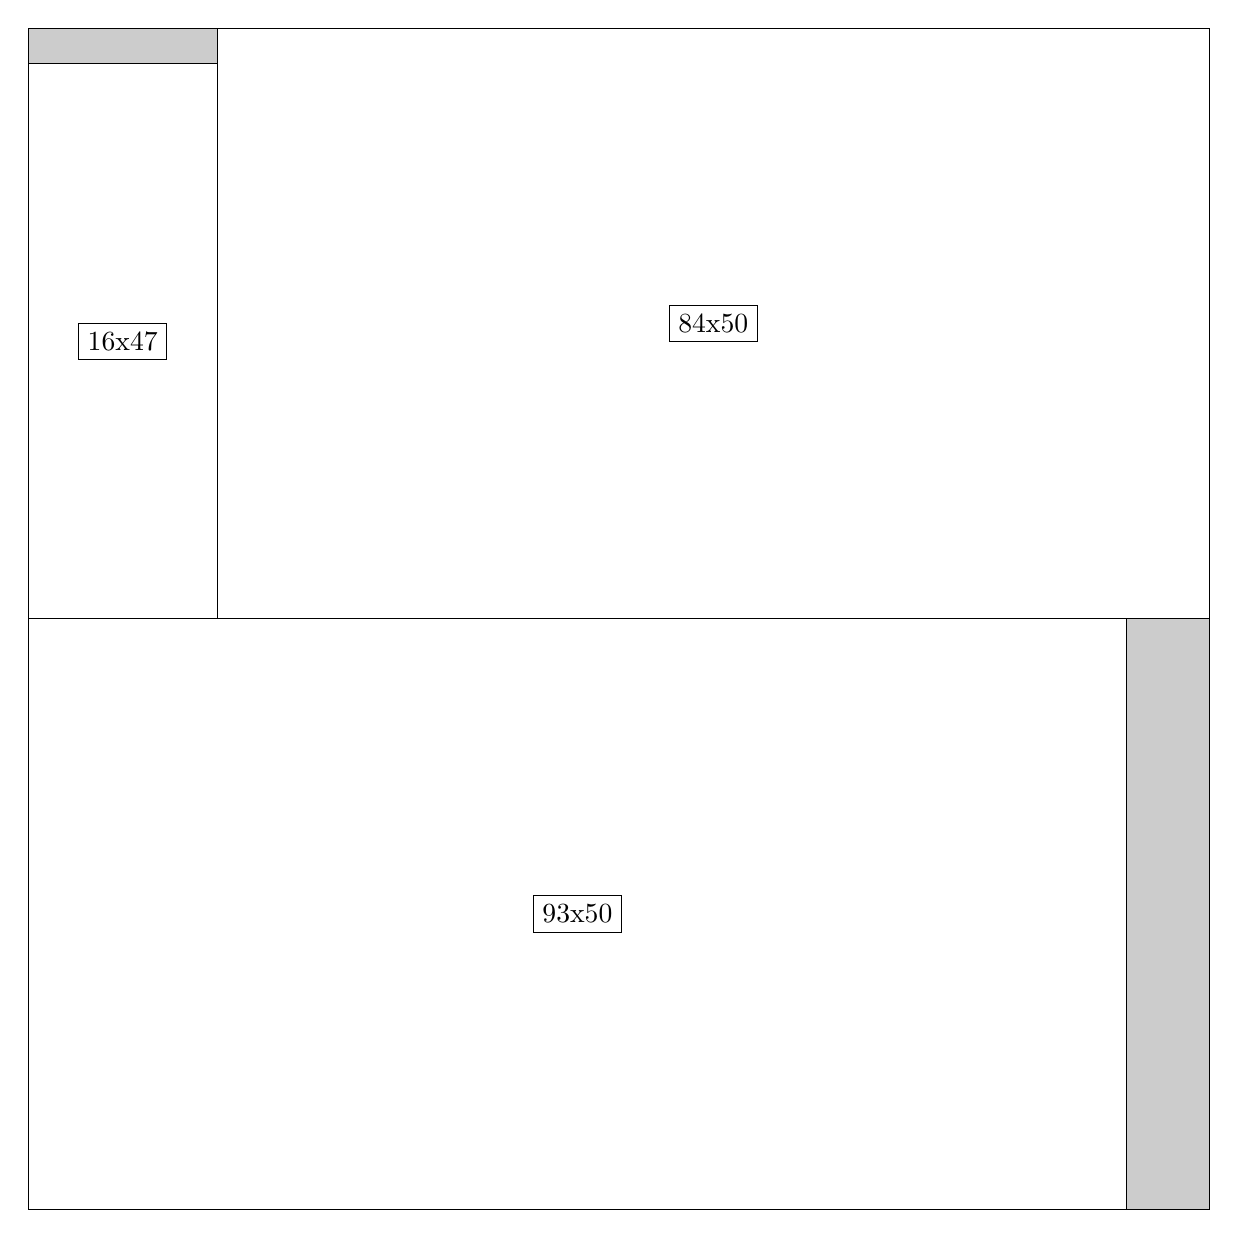
\begin{tikzpicture}[shorten >=1pt,scale=1.0,every node/.style={scale=1.0},->]
\tikzstyle{vertex}=[circle,fill=black!25,minimum size=14pt,inner sep=0pt]
\filldraw[fill=gray!40!white, draw=black] (0,0) rectangle (15.0,15.0);
\foreach \name/\x/\y/\w/\h in {93x50/0.0/0.0/13.95/7.5,84x50/2.4/7.5/12.6/7.5,16x47/0.0/7.5/2.4/7.05}
\filldraw[fill=white!40!white, draw=black] (\x,\y) rectangle node[draw] (\name) {\name} ++(\w,\h);
\end{tikzpicture}


w =93 , h =50 , x =0 , y =0 , v =4650
\par
w =84 , h =50 , x =16 , y =50 , v =4200
\par
w =16 , h =47 , x =0 , y =50 , v =752
\par
\newpage


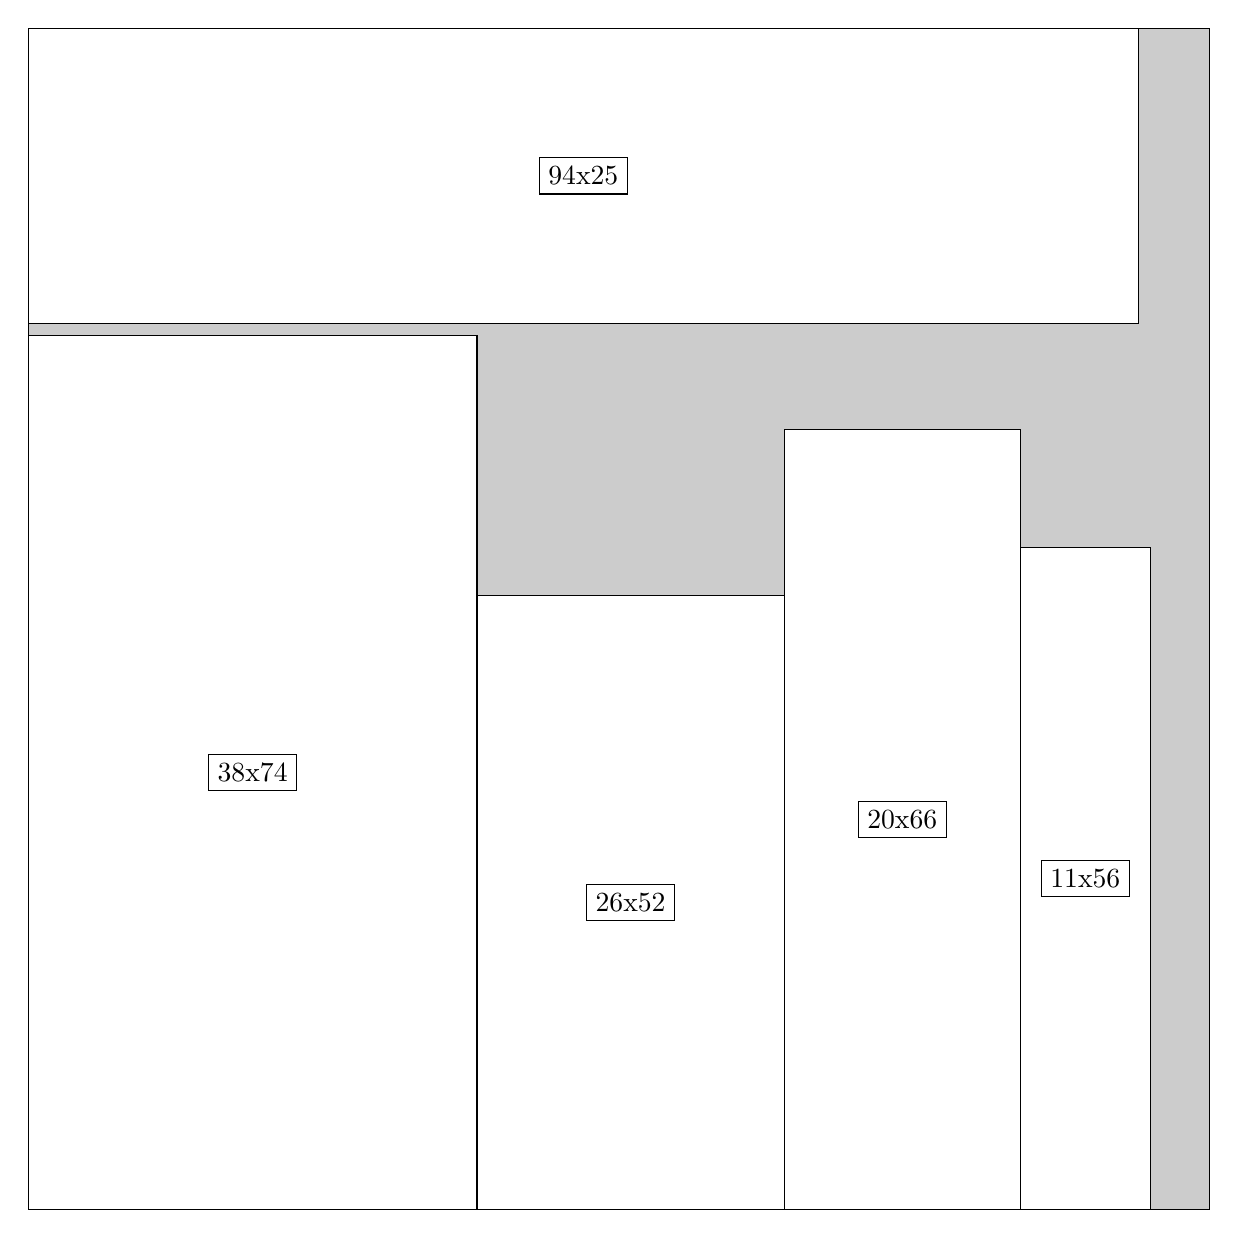
\begin{tikzpicture}[shorten >=1pt,scale=1.0,every node/.style={scale=1.0},->]
\tikzstyle{vertex}=[circle,fill=black!25,minimum size=14pt,inner sep=0pt]
\filldraw[fill=gray!40!white, draw=black] (0,0) rectangle (15.0,15.0);
\foreach \name/\x/\y/\w/\h in {38x74/0.0/0.0/5.7/11.1,94x25/0.0/11.25/14.1/3.75,26x52/5.7/0.0/3.9/7.8,20x66/9.6/0.0/3.0/9.9,11x56/12.6/0.0/1.65/8.4}
\filldraw[fill=white!40!white, draw=black] (\x,\y) rectangle node[draw] (\name) {\name} ++(\w,\h);
\end{tikzpicture}


w =38 , h =74 , x =0 , y =0 , v =2812
\par
w =94 , h =25 , x =0 , y =75 , v =2350
\par
w =26 , h =52 , x =38 , y =0 , v =1352
\par
w =20 , h =66 , x =64 , y =0 , v =1320
\par
w =11 , h =56 , x =84 , y =0 , v =616
\par
\newpage


\end{document}